\documentclass[12pt]{article}
\usepackage{dsfont}
\usepackage{textcomp}
\usepackage{amsmath}
\usepackage{amssymb}
\usepackage{graphicx}
\usepackage{array}


\begin{document}


\title{Solutions to Sheet 10}
\author{Lukas Drexler, Leif Van Holland \\ \\
\textsc{Pattern Matching and Machine Learning} \\
\textsc{for Audio Signal Processing}}
\maketitle

\section*{Exercise 10.1}
\begin{center}
\begin{tabular}{c|c|c|c|c}
    $p$ & $F_{\text{pitch}}(p)$ & $F_{\text{pitch}}(p-0.5)$ & $F_{\text{pitch}}(p+0.5)$ & $BW(p)$ \\
    \hline
    60 & 261,63 & 254,18 & 269,29 & 7,67 \\
    61 & 277,18 & 269,29 & 285,30 & 8,12 \\
    62 & 293,66 & 285,30 & 302,27 & 8,61 \\
    63 & 311,13 & 302,27 & 320,24 & 9,12 \\
    64 & 329,63 & 320,24 & 339,29 & 9,66 \\
    65 & 349,23 & 339,29 & 359,46 & 10,23 \\
    66 & 369,99 & 359,46 & 380,84 & 10,84 \\
    67 & 392,00 & 380,84 & 403,48 & 11,49 \\
    68 & 415,30 & 403,48 & 427,47 & 12,17 \\
    69 & 440,00 & 427,47 & 452,89 & 12,89 \\
    70 & 466,16 & 452,89 & 479,82 & 13,66 \\
    71 & 493,88 & 479,82 & 508,36 & 14,47 \\
    72 & 523,25 & 508,36 & 538,58 & 15,33

\end{tabular}
\end{center}

\section*{Exercise 10.3}
\subsection*{b)}
    \begin{center}
        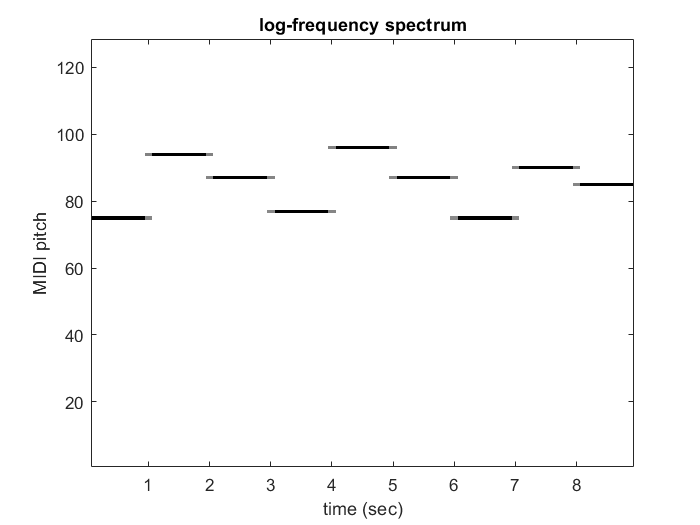
\includegraphics[width=\linewidth]{logspectrum}
    \end{center}

\subsection*{c)}
\begin{center}
    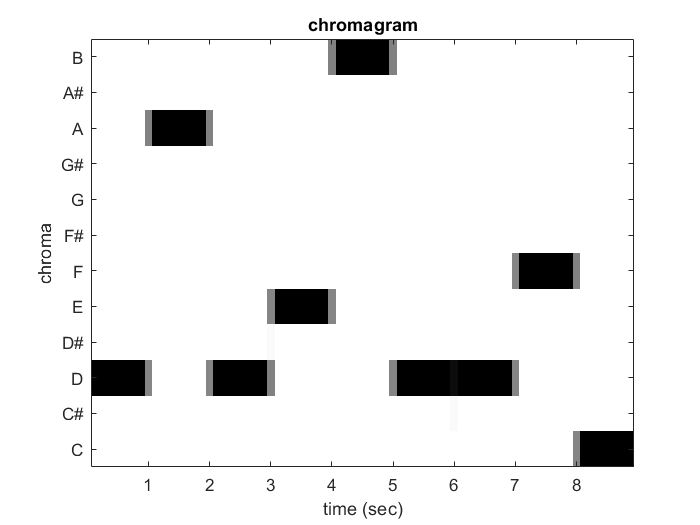
\includegraphics[width=\linewidth]{chromagram}
\end{center}

\end{document}